%!TEX root = main.tex
\section{Background}
\label{sec:background}
\subsection{Synchronous and Asynchronous Pipeline Parallelism}
\emph{Pipeline parallelism} can be categorized based on how model parameters are updated:
\emph{Synchronous Pipeline Parallelism} and \emph{Asynchronous Pipeline Parallelism}.
\emph{SPP} operates similarly to synchronous parameter updates in single-GPU training,
where the computation of the next mini-batch does not begin until
the backward propagation and parameter updates of the current mini-batch are complete.
A notable example of \emph{SPP} is GPipe~\cite{huangGpipeEfficientTraining2019}, proposed by Huang et al., as shown in Figure~\ref{subfig:gpipe}.
In the figure, each small rectangle represents the forward and backward computations of a micro-batch,
with the number inside indicating the micro-batch index.
The pipeline spans four GPUs, with an equal number of micro-batches fed into the pipeline.
However, \emph{SPP} suffers from low GPU utilization due to a synchronization barrier before the next mini-batch can start,
leading to pipeline bubbles (idle GPU time) shown as the blank areas in Figure~\ref{subfig:gpipe}.
In pipeline parallelism,
activation and gradient memory communication can overlap with computation.
Since the size of activation values and gradients is generally smaller than the full model parameters
and only needs to be transferred between adjacent stages,
the communication overhead is typically the lowest among the three parallelism methods.
This approach can potentially reduce communication costs by up to 95\%~\cite{narayananPipeDreamGeneralizedPipeline2019}.

To address the low GPU utilization in \emph{SPP}, PipeDream~\cite{narayananPipeDreamGeneralizedPipeline2019}
introduces an \emph{APP} method with a 1F1B (one forward, one backward) scheduling mechanism to enhance GPU utilization.
As shown in Figure ~\ref{subfig:pipedream}, PipeDream begins with a warm-up phase to initialize the pipeline,
requiring the first $(\ell-x)$ micro-batches in stage $x$ to be fed into the pipeline before the 1F1B scheduling can begin,
in which $\ell$ represents the number of pipeline stages.
To ensure parameter consistency during both the forward and backward passes within the same micro-batch,
multiple versions of parameters must be maintained.
Specifically, $(\ell-x)$ replicas of parameters are stored at stage $x$,
meaning earlier stages require additional GPU memory to hold these replicas.
DAPPLE~\cite{fanDAPPLEPipelinedData2021} extends the 1F1B scheduling approach from PipeDream to GPipe,
optimizing the efficiency of synchronous pipeline parallelism.
Recent works~\cite{sunAdaPipeOptimizingPipeline2024,zhaoVPipeVirtualizedAcceleration2022,liChimeraEfficientlyTraining2021,kimBPipeMemoryBalancedPipeline2023}
have focused on further optimizing pipeline parallelism,
generally building on the 1F1B computation scheduling approaches.
\begin{figure}[htb]
  \centering
  % \hspace{-0.7cm}
  \subfigure[Synchornous Pipeline Parallel — GPipe]{
    \centering
    \label{subfig:gpipe}
    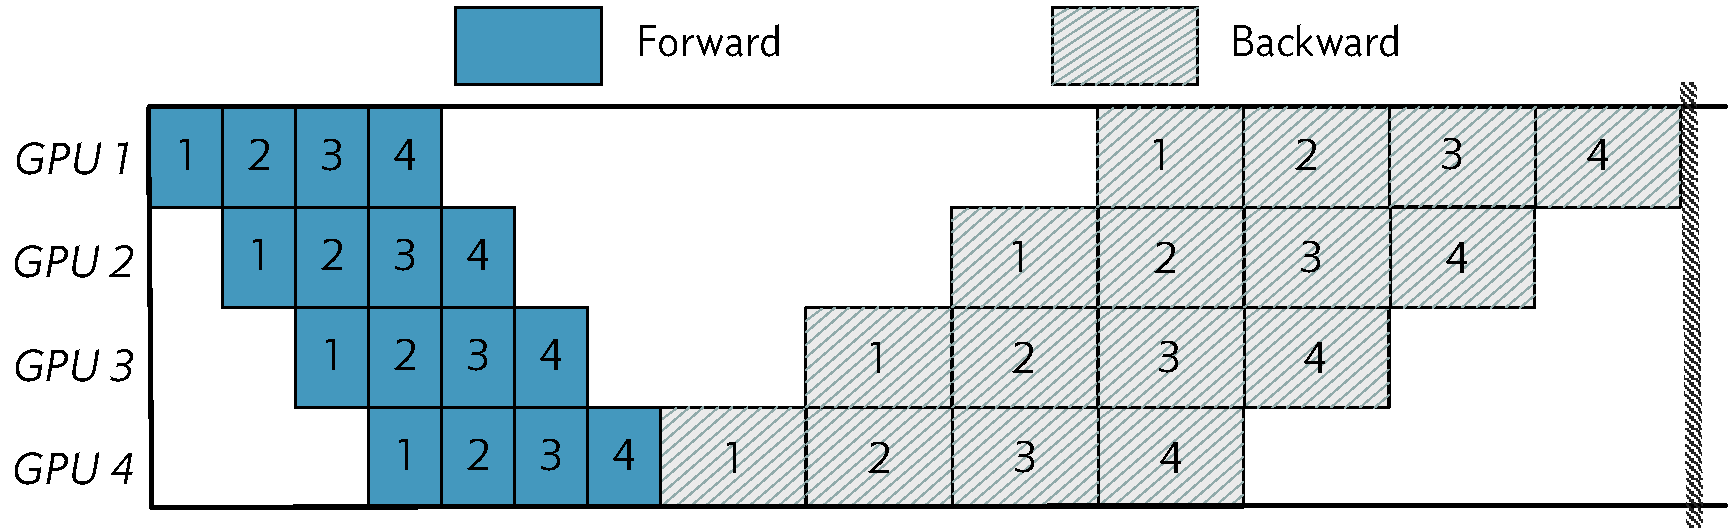
\includegraphics[width=1.0\linewidth]{GPipe-exec.pdf}
  }
  \subfigure[Asynchronous Pipeline Parallel — PipeDream]{
    \centering
    \label{subfig:pipedream}
    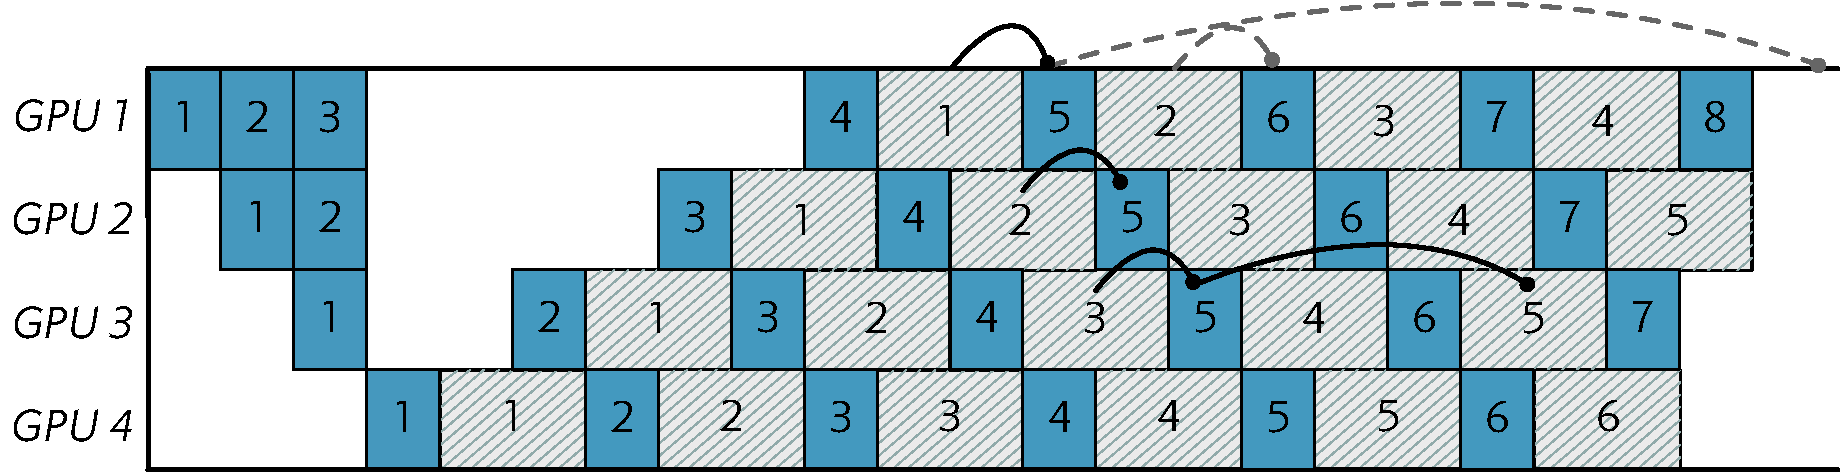
\includegraphics[width=1.0\linewidth]{PipeDream-exec.pdf}
  }
  \caption{Synchornous and Asynchronous Pipeline Parallel Execution}
  \label{fig:pp-exec}
\end{figure}

\subsection{Swap and Recomputation}
Previous works~\cite{rhuVDNNVirtualizedDeep2016,chenTrainingDeepNets2016,wangSuperneuronsDynamicGPU2018,pengCapuchinTensorbasedGPU2020}
on memory optimization for deep learning training have demonstrated that \emph{memory swapping} and \emph{recomputation}
(also known as activation checkpointing) are effective strategies for reducing memory footprint.
Both techniques exploit the time gap between two accesses to the same activation memory during forward and backward propagation.
\emph{Swapping} uses CPU memory as external storage to extend GPU memory capacity
by offloading activation data to the CPU during the forward pass and copying it back to the GPU during the backward pass.
vDNN~\cite{rhuVDNNVirtualizedDeep2016} is the pioneer of this approach.
Chen et al.~\cite{chenTrainingDeepNets2016} introduced activation checkpointing,
which discards activation memory during the forward pass and recomputes it during the backward pass,
adding around 30\% overhead to overall training.
SuperNeurons~\cite{wangSuperneuronsDynamicGPU2018} and Capuchin~\cite{pengCapuchinTensorbasedGPU2020}
proposed dynamic strategies that combine swapping and recomputation to further
reduce memory footprint while maintaining performance.
Wahib et al.~\cite{wahibScalingDistributedDeep2020} extended swap-based optimizations to distributed training environments.
For pipeline parallelism, GPipe integrates recomputation, while vPipe~\cite{zhaoVPipeVirtualizedAcceleration2022}
introduces an iterative pipeline partitioning algorithm that jointly considers swapping, recomputation, and partitioning.
AdaPipe~\cite{sunAdaPipeOptimizingPipeline2024} further refines this approach with a two-step
dynamic programming algorithm for pipeline partitioning and recomputation within the 1F1B pipeline parallel scheduling framework.
